%% UICTHESI.TEX — MS Project Report
%% Author: Archit Rathod
%% University of Illinois at Chicago
%
\documentclass{bin/uicthesi}

% helpers
\usepackage{url}
\usepackage{cite}
\usepackage{amsthm}
\usepackage{lipsum}
\usepackage{dsfont}
\usepackage{hhline}
\usepackage{amsmath}
\usepackage{amssymb}
\usepackage{calligra}
\usepackage{graphicx}
\usepackage{epstopdf}
\usepackage{makecell}
\usepackage{multirow}
\usepackage{titletoc}
\usepackage{thmtools}
\usepackage{extarrows}
\usepackage{longtable}
\usepackage{subfigure}
%\usepackage[sectionbib, numbers]{natbib}
%\usepackage{chapterbib}
\usepackage[dvipsnames]{xcolor}
\usepackage[final]{pdfpages}
\usepackage[T1]{fontenc}
\usepackage{algpseudocode}
\usepackage[inline]{enumitem}
\usepackage[chapter]{algorithm}
\usepackage[newparttoc]{titlesec}

% Additional packages for FairLint-DL project report
\usepackage{booktabs}
\usepackage{float}
\usepackage{array}
\usepackage{caption}
\usepackage{listings}
\usepackage{hyperref}

% Code listing colors and style
\definecolor{codebg}{rgb}{0.95,0.95,0.97}
\definecolor{codegreen}{rgb}{0,0.5,0}
\definecolor{codegray}{rgb}{0.5,0.5,0.5}
\definecolor{codepurple}{rgb}{0.58,0,0.82}

\lstdefinestyle{mystyle}{
    backgroundcolor=\color{codebg},
    commentstyle=\color{codegreen},
    keywordstyle=\color{blue},
    numberstyle=\tiny\color{codegray},
    stringstyle=\color{codepurple},
    basicstyle=\ttfamily\footnotesize,
    breakatwhitespace=false,
    breaklines=true,
    captionpos=b,
    keepspaces=true,
    numbers=left,
    numbersep=5pt,
    showspaces=false,
    showstringspaces=false,
    showtabs=false,
    tabsize=2,
    frame=single,
    framesep=5pt,
    xleftmargin=15pt,
    xrightmargin=5pt
}
\lstset{style=mystyle}

\hypersetup{
    colorlinks=true,
    linkcolor=blue!70!black,
    citecolor=green!50!black,
    urlcolor=blue!60!black
}


%\usepackage{ifpdf}
%\usepackage{array}
%\usepackage{tabularx}
%\usepackage{amsbsy}
%\usepackage{amscd}
%\usepackage{float}
%\usepackage{refcount}
%\usepackage{bibentry}

%\usepackage{biblatex}
%\usepackage{bm}
%\usepackage{blindtext}
%\usepackage{color}
%\usepackage{booktabs}
%\usepackage{enumerate}
%\usepackage{cellspace}
%\usepackage[inline]{enumitem}
\input{bin/settings.tex}
\input{bin/symbols.tex}

%% Override \maketitle to say PROJECT REPORT instead of THESIS
%% and Evaluation Committee instead of Defense Committee
\makeatletter
\def\maketitle{%
   \begin{titlepage}
      \centering
      \thispagestyle{empty}
      \c@page=2
      \vbox to 0pt{%
         \begin{center}
            \large\transparentbold\@title
         \end{center}\vss}
      \vfill
      \begin{singlespace}
         BY
         \vskip\baselineskip
         \begin{tabular}{c}
            \@upauthor\\\@pdegrees
         \end{tabular}
         \vfill
         \vbox to 0pt{\vss
            \begin{center}
               \vskip \baselineskip
               PROJECT REPORT\\
               \vskip \baselineskip
               Submitted as partial fulfillment of the requirements\\
               for the degree of \@degree\\
               in the Graduate College of the\\
               University of Illinois at Chicago, \@date
               \vskip 2\baselineskip
               Chicago, Illinois
               \vskip 3\baselineskip
            \end{center}}
         \begin{flushleft}
         Evaluation Committee:\\
         \vskip \baselineskip
         \begin{minipage}{.1\textwidth}
         \end{minipage}
         \hfill
         \begin{minipage}{.9\textwidth}
            \@committee
         \end{minipage}
        \end{flushleft}
      \end{singlespace}
   \end{titlepage}}
\makeatother

% Declarations for front matter
\title{FairLint-DL: Deep Learning-Based Fairness Debugging for Machine Learning Datasets}
\author{Archit Rathod}
\pdegrees{B.S. in Computer Science}
\degree{Master of Science in Computer Science}
\committee{Saeid Tizpaz-Niari, Advisor \\
	Abolfazl Asudeh, Secondary Evaluator}
\makeatletter

\begin{document}
\maketitle
\copyrightpage

% supplementary pages
\acknowledgementsI would like to thank my advisor, Professor Saeid Tizpaz-Niari, for his invaluable guidance, support, and expertise throughout the development of this project. His insights into fairness testing and software engineering for AI provided the foundational direction for FairLint-DL.

I also thank Professor Abolfazl Asudeh for serving as the secondary evaluator and providing thoughtful feedback on this work.

\vspace{60pt}
\hfill AR

\tableofcontents
\listoftables
\listoffigures
\summaryAs machine learning systems are increasingly deployed in socially critical domains---including criminal justice, lending, healthcare, and hiring---ensuring that these systems do not discriminate based on legally protected attributes such as race, sex, and age has become a paramount concern. Existing fairness analysis tools predominantly operate as post-training evaluation frameworks, requiring practitioners to complete the full model development lifecycle before assessing bias. This report presents \textbf{FairLint-DL}, a Visual Studio Code extension that implements a \emph{shift-left} approach to fairness testing by enabling pre-training, IDE-native bias detection directly on tabular datasets.

FairLint-DL trains a configurable deep neural network as a proxy model and applies information-theoretic \emph{Quantitative Individual Discrimination} (QID) metrics---grounded in Shannon entropy and min-entropy---to quantify the causal influence of protected attributes on model predictions. The system implements a two-phase gradient-guided search algorithm for discovering discriminatory instances, a causal debugging pipeline that localizes bias to specific network layers and neurons via sensitivity analysis, and dual explainability engines using SHAP (SHapley Additive exPlanations) and LIME (Local Interpretable Model-agnostic Explanations) for feature-level attribution.

Evaluation on the Adult Census Income dataset (32,561 records, 14 features) reveals severe fairness concerns: 95.8\% of analyzed instances exhibit QID above the 0.1-bit significance threshold, with a mean QID of 0.640 bits. The disparate impact ratio of 0.581 violates the four-fifths legal standard, and group fairness metrics confirm systematic disparities across demographic parity, equalized odds, and equal opportunity for the protected attributes of sex, race, age, and national origin. Causal debugging identifies Layer~2 (32 neurons) as the most bias-sensitive layer, with Neuron~30 exhibiting the highest impact score of 1.362. The composite fairness score of approximately 41 out of 100 rates the dataset as ``Concerning.'' FairLint-DL produces these results within 12~seconds on cached models, demonstrating the feasibility of integrating comprehensive fairness analysis into the developer workflow without significant overhead.


% chapters
\chapter{Introduction}
\label{ch:introduction}

\section{Motivation}

The proliferation of deep neural networks (DNNs) in high-stakes decision-making systems has introduced significant concerns regarding algorithmic fairness. Instances of such AI-assisted software include systems deciding on recidivism risk~\cite{dice}, software predicting benefit eligibility, and tools deciding whether to audit a given taxpayer. The DNN-based software development process, driven by the principle of information bottleneck~\cite{dice}, involves a delicate balancing act between over-fitting and detecting useful, parsimonious patterns. It is therefore not surprising that such solutions often encode and amplify pre-existing biases in the training data. Worse, improper training may even introduce biases not present in the training data or irrelevant to the decision-making task. The resulting fairness defects may not only disadvantage protected groups but may also violate statutory requirements such as the Civil Rights Act's disparate impact provisions and the EU AI Act's fairness mandates.

From a philosophical perspective, fairness in machine learning exists at the intersection of multiple frameworks: utilitarianism (maximizing overall welfare), egalitarianism (reducing inequality), and Rawlsian justice (max--min fairness)~\cite{mentalmap}. The legal landscape further distinguishes between \emph{disparate treatment}---intentional discrimination based on protected attributes---and \emph{disparate impact}---facially neutral policies that disproportionately affect protected groups. FairLint-DL addresses both dimensions through its combination of individual-level counterfactual analysis and group-level statistical fairness metrics.

\section{The Shift-Left Fairness Testing Paradigm}

Current fairness tools predominantly operate in a post-training paradigm: practitioners must complete the full model development lifecycle---data collection, preprocessing, feature engineering, model selection, hyperparameter tuning, and training---before evaluating bias. Tools such as IBM's AI Fairness 360, Google's What-If Tool, and Microsoft's Fairlearn~\cite{evt, fairlearn, Wexler_2019, bellamy2019} provide valuable post-hoc analysis but require significant upfront investment before fairness issues are identified.

FairLint-DL introduces a \emph{shift-left} approach to fairness testing, analogous to shift-left testing in software engineering. By integrating directly into the developer's IDE as a VS Code extension, FairLint-DL enables practitioners to assess dataset bias \emph{before} committing to a specific model architecture or training pipeline. This approach offers several advantages: bias detected early is cheaper to fix (modifying datasets is less expensive than retraining models), the feedback loop is tighter (results appear in the same environment where code is written), and the barrier to fairness testing is lowered (no separate tool or workflow is required).

\section{Problem Statement}

Given a tabular dataset $A = (A_X, A_Z)$ partitioned into non-protected variables $X = X_1 \times X_2 \cdots \times X_n$ (such as profession, income, and education) and protected variables $Z = Z_1 \times Z_2 \cdots \times Z_r$ (such as race, sex, and age), and a DNN $\mathcal{D}: X \times Z \rightarrow [0,1]^t$ trained on $A$, FairLint-DL seeks to:

\begin{enumerate}[label=(\arabic*)]
    \item \textbf{Quantify} the amount of protected information used in deriving outcomes, measured in bits via Shannon entropy and min-entropy;
    \item \textbf{Search} the input space for discriminatory instances that maximize the use of protected information;
    \item \textbf{Localize} the bias to specific layers and neurons within the DNN through causal debugging; and
    \item \textbf{Explain} which input features drive the bias through SHAP and LIME attribution methods.
\end{enumerate}

\section{Contributions}

The key contributions of this project are:

\begin{enumerate}[label=(\arabic*)]
    \item An IDE-integrated fairness testing tool that implements the shift-left paradigm for bias detection in machine learning datasets.
    \item Implementation of information-theoretic QID metrics combining Shannon entropy and min-entropy for quantitative discrimination measurement.
    \item A gradient-guided two-phase search algorithm for discovering discriminatory instances in the input space.
    \item Causal debugging that localizes bias to specific DNN layers and neurons using sensitivity analysis and activation magnitude scoring.
    \item Dual explainability via SHAP and LIME with cross-method validation for robust feature attribution.
    \item A composite fairness scoring system integrating individual-level QID and group-level fairness metrics (Demographic Parity, Equalized Odds, Equal Opportunity).
    \item Comprehensive empirical evaluation on the Adult Census Income dataset demonstrating severe and pervasive bias across multiple protected attributes.
\end{enumerate}

\section{Report Organization}

The remainder of this report is organized as follows. Chapter~\ref{ch:background} surveys the theoretical foundations and related work. Chapter~\ref{ch:architecture} presents the system architecture and design. Chapter~\ref{ch:methodology} details the algorithmic methodology. Chapter~\ref{ch:implementation} describes the implementation. Chapter~\ref{ch:evaluation} presents the experimental evaluation on the Adult Census dataset. Chapter~\ref{ch:discussion} discusses findings and limitations. Chapter~\ref{ch:conclusion} concludes with directions for future work.

\chapter{Background and Related Work}
\label{ch:background}

\section{Fairness Definitions}

The machine learning fairness literature distinguishes between several families of fairness definitions~\cite{mentalmap}.

\subsection{Individual Fairness}

Individual fairness, formalized by Dwork et al.\ (2012), requires that similar individuals receive similar outcomes. Formally, for a Lipschitz-continuous mapping $M$, the requirement is $d_Y(M(x), M(x')) \leq L \cdot d_X(x, x')$, where $d_X$ and $d_Y$ are distance metrics in the input and output spaces, respectively. \emph{Counterfactual fairness} extends this notion causally: the prediction should remain unchanged if the protected attribute were counterfactually altered. FairLint-DL's QID metric operationalizes this notion by measuring the entropy of predictions across counterfactual variations of protected attributes.

\subsection{Group Fairness}

Group fairness (statistical fairness) requires parity of some statistical measure across demographic groups~\cite{mentalmap}. Three prominent criteria are:

\textbf{Demographic Parity} (Independence-Based): $P(\hat{Y}=1 | A=a) = P(\hat{Y}=1 | A=b)$, requiring equal positive prediction rates across groups.

\textbf{Equalized Odds} (Separation-Based): $P(\hat{Y}=1 | A=a, Y=y) = P(\hat{Y}=1 | A=b, Y=y)$ for all $y$, requiring equal true positive rates and false positive rates.

\textbf{Equal Opportunity}: A relaxation of Equalized Odds that requires only equal true positive rates: $P(\hat{Y}=1 | A=a, Y=1) = P(\hat{Y}=1 | A=b, Y=1)$.

Kleinberg et al.\ (2016) proved an impossibility theorem showing that calibration, equalized odds, and unequal base rates cannot be simultaneously satisfied~\cite{mentalmap}, motivating the use of multiple complementary metrics as implemented in FairLint-DL.

\subsection{Causal Fairness}

Causal fairness, grounded in Pearl's framework of structural causal models, requires that the prediction is causally independent of protected attributes. Path-specific fairness further distinguishes between fair and unfair causal pathways, blocking only the latter. FairLint-DL's causal debugging algorithm traces the causal influence of protected attributes through the network's internal structure.

\section{Information-Theoretic Fairness Testing: DICE}

The DICE framework~\cite{dice} introduced Quantitative Individual Discrimination (QID) as an information-theoretic characterization of discrimination. QID is defined as the amount of protected information---characterized by Shannon entropy and min-entropy---used in deriving an outcome. A zero QID value implies the absence of individual discrimination, while higher values indicate greater reliance on protected information. DICE also introduced a causal debugging algorithm (Algorithm~2 in~\cite{dice}) that uses interventions on neuron activations to localize layers and neurons with significant causal effects on QID. On the Adult Census dataset, DICE discovered 36 clusters from 14 initial clusters, generating 230,593 test cases with QID values up to 5.3 bits, and identified the second layer as the most bias-sensitive.

\section{NeuFair: Neural Network Fairness Repair}

NeuFair~\cite{neufair} extends the search algorithm for finding discriminatory instances using a two-phase global-local approach with gradient-based optimization. NeuFair formulates fairness repair as a simulated annealing optimization problem over neuron dropout configurations, using a cost function that balances Equalized Odds Difference (EOD) minimization with F1 score preservation. NeuFair substantially outperforms DICE in improving fairness through multi-neuron dropout strategies.

\section{Extreme Value Theory for Fairness}

The EVT framework~\cite{evt_cain} applies extreme value theory to model the worst-case convergence times and extreme counterfactual discrimination in ML systems. By fitting Generalized Extreme Value (GEV) distributions to the tail of discrimination measurements, EVT provides probabilistic guarantees on worst-case bias scenarios, complementing the average-case analysis of QID.

\section{FairLay-ML: GUI MLOps Pipeline}

FairLay-ML~\cite{fairlayml} presents a GUI MLOps pipeline for fairness debugging that allows users to upload data and ML models for counterfactual testing. It implements feature interaction visualization, model logic explanation via LIME, and manual manipulation of test cases. FairLint-DL extends this paradigm by integrating directly into the IDE and adding deep learning-specific analysis capabilities including causal debugging and gradient-guided search.

\section{Explainability Methods}

\textbf{SHAP} (SHapley Additive exPlanations) computes the exact contribution of each feature to every prediction using game-theoretic Shapley values. The KernelExplainer variant is model-agnostic and operates on arbitrary prediction functions.

\textbf{LIME} (Local Interpretable Model-agnostic Explanations) approximates the model locally around each instance with a simple linear model by generating perturbations and observing prediction changes. LIME provides complementary local explanations that can reveal context-dependent bias patterns.

\chapter{System Architecture and Design}
\label{ch:architecture}

\section{Client-Server Architecture}

FairLint-DL operates as a client-server application with two primary components communicating over HTTP/REST on \texttt{localhost:8765}:

\begin{itemize}
    \item \textbf{VS Code Extension (Client):} Written in TypeScript, the extension handles all user interaction, file system access, WebView dashboard rendering with Plotly.js charts, and manages the lifecycle of the Python backend.
    \item \textbf{Python FastAPI Backend (Server):} Hosts the PyTorch models and all analysis algorithms, including data preprocessing, model training, QID computation, causal debugging, discriminatory instance search, and SHAP/LIME explainability.
\end{itemize}

\begin{figure}[H]
    \centering
    \includegraphics[width=0.95\textwidth]{images/fairlint-dl-architecture.png}
    \caption{FairLint-DL client-server architecture overview.}
    \label{fig:architecture}
\end{figure}

When the extension activates, it spawns the Python backend as a child process via \texttt{python -m uvicorn bias\_server:app --port 8765} and polls the health endpoint (\texttt{GET /}) until the server responds, retrying up to 15 times with 1-second intervals.

\section{REST API Endpoints}

The backend exposes seven endpoints that correspond to the six-step analysis pipeline:

\begin{table}[H]
\centering
\caption{FairLint-DL REST API endpoints.}
\label{tab:api}
\begin{tabular}{@{}llp{7cm}@{}}
\toprule
\textbf{Endpoint} & \textbf{Method} & \textbf{Description} \\
\midrule
\texttt{/} & GET & Health check \\
\texttt{/columns} & POST & Returns column names, sample data, auto-detected sensitive features \\
\texttt{/train} & POST & Trains proxy model (or loads from cache); supports \texttt{force\_retrain} \\
\texttt{/activations} & POST & Returns PCA/t-SNE reduced layer activations \\
\texttt{/analyze} & POST & Computes QID metrics and group fairness metrics \\
\texttt{/search} & POST & Runs global/local discriminatory instance search \\
\texttt{/debug} & POST & Performs layer and neuron sensitivity analysis \\
\texttt{/explain} & POST & Generates batch SHAP/LIME explanations \\
\texttt{/explain-instance} & POST & Single-instance LIME explanation (by index or custom values) \\
\bottomrule
\end{tabular}
\end{table}

\section{Project Structure}

The codebase is organized into the following directory structure:

\begin{lstlisting}[language={}, caption={FairLint-DL project structure.}]
fairlint-dl/
+-- python_backend/        # Analysis Server
|   +-- analyzers/         # Core Algorithmic Logic
|   |   +-- causal_debugger.py    # Layer/Neuron attribution
|   |   +-- qid_analyzer.py       # Entropy-based metrics
|   |   +-- search.py             # Gradient-guided search
|   |   +-- explainability.py     # SHAP and LIME explanations
|   |   +-- group_fairness.py     # DP, EO, EOpp metrics
|   |   +-- internal_space.py     # PCA/t-SNE visualization
|   +-- models/
|   |   +-- fairness_dnn.py       # PyTorch DNN definition
|   +-- utils/
|   |   +-- data_loader.py        # CSV loading, encoding, scaling
|   |   +-- model_cache.py        # SHA-256 caching system
|   +-- bias_server.py            # FastAPI entry point
+-- src/                   # VS Code Extension Source
|   +-- extension.ts              # Main entry point
|   +-- analysis/pipeline.ts      # 6-step pipeline orchestration
|   +-- webview/
|       +-- results.ts            # WebView panel management
|       +-- htmlBuilder.ts        # Dashboard HTML generation
|       +-- charts.ts             # Plotly.js chart rendering
|       +-- scoring.ts            # Composite fairness score
+-- package.json                  # Extension manifest
\end{lstlisting}

\section{Six-Step Analysis Pipeline}

The analysis follows a sequential six-step pipeline orchestrated by \texttt{pipeline.ts}:

\begin{enumerate}
    \item \textbf{Model Training:} Train (or load cached) DNN proxy model on the dataset.
    \item \textbf{Internal Space Visualization:} Extract and reduce layer activations via PCA.
    \item \textbf{QID Analysis:} Compute Shannon entropy QID, min-entropy QID, disparate impact, and group fairness metrics across all protected attributes~\cite{dice}.
    \item \textbf{Discriminatory Instance Search:} Gradient-guided global search followed by perturbation-based local search~\cite{dice, neufair}.
    \item \textbf{Causal Debugging:} Layer sensitivity analysis followed by neuron-level impact scoring~\cite{dice}.
    \item \textbf{Explainability:} Batch SHAP (KernelExplainer on log-odds) and LIME explanations with interactive per-instance explorer~\cite{kamolov2025, wang2024}.
\end{enumerate}

\chapter{Algorithmic Methodology}
\label{ch:methodology}

\section{Deep Neural Network Proxy Model}

FairLint-DL trains a feedforward DNN as a proxy model to serve as a ``fairness oracle.'' The default architecture uses a 6-layer fully-connected network with $\langle 64, 32, 16, 8, 4, 2 \rangle$ neurons, following the architecture used in prior fairness testing literature~\cite{dice, neufair}. Each hidden layer applies Batch Normalization, ReLU activation, and Dropout ($p=0.2$) for regularization. The model is trained with CrossEntropyLoss and the Adam optimizer (learning rate $= 0.001$) with early stopping (patience $= 10$ epochs).

The rationale for training a DNN rather than using statistical tests on raw data is fourfold: (1) the network learns non-linear decision boundaries revealing complex feature interactions; (2) counterfactual analysis requires a differentiable model; (3) gradient-based search requires backpropagation; and (4) causal debugging traces bias through internal representations.

\section{Quantitative Individual Discrimination (QID)}

QID measures the causal influence of protected attributes on the model's prediction using information-theoretic metrics.

\subsection{Shannon Entropy QID}

Given an individual with non-protected value $X = x$ and protected attribute $Z = z$, the Shannon entropy QID quantifies the uncertainty in prediction introduced by varying $Z$ while keeping $X$ constant:

\begin{equation}
    \text{QID}_{\text{Shannon}}(x) = H(Y | X = x) = -\sum_{y} \bar{P}(Y=y | x) \log_2 \bar{P}(Y=y | x)
    \label{eq:qid_shannon}
\end{equation}

where $\bar{P}(Y=y | x)$ is the average prediction probability across all counterfactual variations of the protected attributes. The computation proceeds as follows: (1) generate counterfactuals $x'$ by modifying protected attributes of $x$; (2) compute predictions $P(Y | x')$ for all counterfactuals; (3) calculate the entropy of the average prediction distribution. A QID of 0 bits implies perfect fairness, while QID approaching 1 bit (for binary classification) indicates maximum discrimination where the protected attribute completely determines the outcome.

\subsection{Min-Entropy QID and Disparate Impact}

FairLint-DL also computes a worst-case metric via min-entropy and the \emph{disparate impact ratio}:

\begin{equation}
    \text{DI}(x) = \frac{\min_{z} P(\hat{Y}=1 | x, z)}{\max_{z} P(\hat{Y}=1 | x, z)}
    \label{eq:disparate_impact}
\end{equation}

The \emph{four-fifths rule} (80\% rule) establishes that a disparate impact ratio below 0.8 constitutes evidence of adverse impact---a well-established legal standard for employment discrimination under U.S.\ civil rights law.

\section{Gradient-Guided Discriminatory Instance Search}

The search for discriminatory instances is formulated as a two-phase optimization problem, inspired by DICE~\cite{dice} and extended by NeuFair~\cite{neufair}.

\subsection{Phase 1: Global Search (Gradient Ascent)}

The global phase maximizes the QID score directly using gradient ascent. The objective function maximizes the variance of predictions across counterfactuals. Gradients of the QID loss are backpropagated with respect to the input features $x$, yielding an input $x_{\text{global}}$ that maximizes discrimination potential.

\subsection{Phase 2: Local Search (Perturbation)}

The local phase explores the neighborhood of $x_{\text{global}}$ by adding Gaussian noise to non-protected features and filtering neighbors that exceed the QID threshold ($> 0.1$ bits), producing concrete discriminatory instances as evidence.

\section{Causal Debugging}

\subsection{Layer Localization}

Layer localization determines which layer is most sensitive to discriminatory inputs by computing the gradient of layer activations $L_i(x)$ with respect to the input $x$ and aggregating the magnitude of these gradients for known discriminatory instances:

\begin{equation}
    \delta_l = \max_{x \in I} \Delta\left(\mathcal{D}_l(z, x), \mathcal{D}_l(z', x)\right)
    \label{eq:layer_sensitivity}
\end{equation}

where $I$ is the set of discriminatory test cases and $\Delta$ is the $L_1$-norm distance function. A normalized sensitivity score $\rho_l = (\delta_l - \delta_{\max,l}) / (\delta_{\max,l} + 1)$ identifies the layer with the highest relative sensitivity as the bias-critical layer.

\subsection{Neuron Localization}

Within the bias-critical layer, neuron localization identifies individual neurons encoding protected information. Following the Average Causal Difference (ACD) framework from DICE~\cite{dice}, the tool intervenes on each neuron by forcing it active ($n > 0$) or inactive ($n = 0$) and measures the resulting change in QID:

\begin{equation}
    \text{ACD}_{l,j} = \mathbb{E}\left[\text{QID} \mid \text{do}(l, j, v^{>0})\right] - \mathbb{E}\left[\text{QID} \mid \text{do}(l, j, v^{=0})\right]
    \label{eq:acd}
\end{equation}

Neurons with disproportionately high impact scores are candidates for pruning, retraining, or regularization in a fairness remediation workflow.

\section{Group Fairness Metrics}

FairLint-DL complements individual-level QID with three group-level fairness metrics. Groups are defined by the standardized protected attribute value: Group~A ($\leq 0$, at or below the mean) and Group~B ($> 0$, above the mean).

\textbf{Demographic Parity} measures whether positive prediction rates are equal: $\text{DP}_{\text{diff}} = |P(\hat{Y}=1 | A) - P(\hat{Y}=1 | B)|$.

\textbf{Equalized Odds} compares both TPR and FPR: $\text{EO}_{\max} = \max(|\text{TPR}_A - \text{TPR}_B|, |\text{FPR}_A - \text{FPR}_B|)$.

\textbf{Equal Opportunity} focuses solely on TPR equality: $\text{EOpp}_{\text{diff}} = |\text{TPR}_A - \text{TPR}_B|$.

\section{Explainability: SHAP and LIME}

\subsection{SHAP on Log-Odds Space}

A critical design decision: FairLint-DL computes SHAP values on the log-odds (margin) output rather than softmax probabilities. The margin is defined as $\text{margin} = \text{logit}(\text{class}=1) - \text{logit}(\text{class}=0) = \log(P(>50K) / P(\leq 50K))$. This is mathematically important because softmax compresses differences (understating true feature contributions), whereas the log-odds space is linear and preserves the scale of feature effects.

\subsection{LIME Local Explanations}

LIME generates 500 perturbations per instance, fits a local linear model, and identifies the feature conditions with the greatest influence on individual predictions. The interactive LIME explorer allows practitioners to test specific scenarios via custom feature values.

\section{Composite Fairness Score}

The composite score maps to a 0--100 scale with five penalty components:

\begin{equation}
    \text{Score} = 100 - P_{\text{meanQID}} - P_{\text{pctDisc}} - P_{\text{DI}} - P_{\text{maxQID}} - P_{\text{group}}
    \label{eq:score}
\end{equation}

where $P_{\text{meanQID}} = \min(\text{mean\_qid} \times 15, 30)$, $P_{\text{pctDisc}} = \min(\text{pct\_disc} \times 0.3, 30)$, $P_{\text{DI}} = (0.8 - \text{DI}) \times 50$ if $\text{DI} < 0.8$, $P_{\text{maxQID}} = \min(\text{max\_qid} \times 5, 20)$, and $P_{\text{group}} = \min((\overline{\text{DP}_{\text{diff}}} + \overline{\text{EO}_{\max}}) \times 25, 20)$.

\chapter{Implementation}
\label{ch:implementation}

\section{Technology Stack}

\begin{table}[H]
\centering
\caption{FairLint-DL technology stack.}
\label{tab:techstack}
\begin{tabular}{@{}lll@{}}
\toprule
\textbf{Component} & \textbf{Technology} & \textbf{Purpose} \\
\midrule
DNN Framework & PyTorch 2.0+ & Model training, gradient computation \\
Backend Server & FastAPI + Uvicorn & REST API, async request handling \\
Extension Frontend & TypeScript & VS Code extension, WebView dashboard \\
Data Visualization & Plotly.js (CDN) & Interactive charts in WebView \\
Data Processing & Pandas, Scikit-learn & CSV loading, encoding, scaling \\
Explainability & SHAP, LIME & Feature attribution \\
\bottomrule
\end{tabular}
\end{table}

\section{DNN Model Architecture}

The \texttt{FairnessDetectorDNN} class implements a configurable feedforward neural network:

\begin{lstlisting}[language=Python, caption={DNN architecture definition (simplified).}]
class FairnessDetectorDNN(nn.Module):
    def __init__(self, input_dim, hidden_layers=[64,32,16,8,4],
                 num_classes=2, dropout=0.2):
        super().__init__()
        layers = []
        prev_dim = input_dim
        for h in hidden_layers:
            layers.extend([
                nn.Linear(prev_dim, h),
                nn.BatchNorm1d(h),
                nn.ReLU(),
                nn.Dropout(dropout)
            ])
            prev_dim = h
        layers.append(nn.Linear(prev_dim, num_classes))
        self.network = nn.Sequential(*layers)
\end{lstlisting}

For the Adult Census dataset with 14 features, the model contains 3,998 trainable parameters across layers $\langle 64, 32, 16, 8, 4, 2 \rangle$.

\section{Model Caching System}

To avoid redundant retraining, FairLint-DL implements a deterministic SHA-256 caching system. The cache key is computed from six parameters: the SHA-256 hash of the CSV file contents (not the file path), the label column name, the sorted set of sensitive features, hidden layer sizes, number of epochs, and batch size. Any change to these parameters invalidates the cache. Stored artifacts include model weights (\texttt{model.pt}), preprocessor state (\texttt{preprocessor.pkl}), train/validation/test data splits (\texttt{data\_tensors.pt}), and human-readable metadata (\texttt{metadata.json}).

\section{Data Preprocessing}

The \texttt{data\_loader.py} module handles CSV loading with automatic type detection: categorical features are ordinally encoded, continuous features are standardized via \texttt{StandardScaler} (zero mean, unit variance), and the dataset is split into training (70\%), validation (10\%), and test (20\%) partitions. Protected attributes are auto-detected via regex pattern matching against common sensitive feature names (age, gender, sex, race, ethnicity, religion, disability, national origin, marital status).

\section{VS Code Extension Integration}

The extension is activated on Python files or workspaces containing CSV files. Users trigger analysis via the context menu (right-click on a \texttt{.csv} file). The extension presents QuickPick dialogs for selecting the label column, protected attributes, and model architecture. Configurable settings are exposed through VS Code's settings API, including training epochs (default: 30), batch size (default: 32), hidden layer configuration, QID threshold (default: 0.1 bits), maximum analysis samples (default: 500), server port, and visualization theme.

\begin{figure}[H]
    \centering
    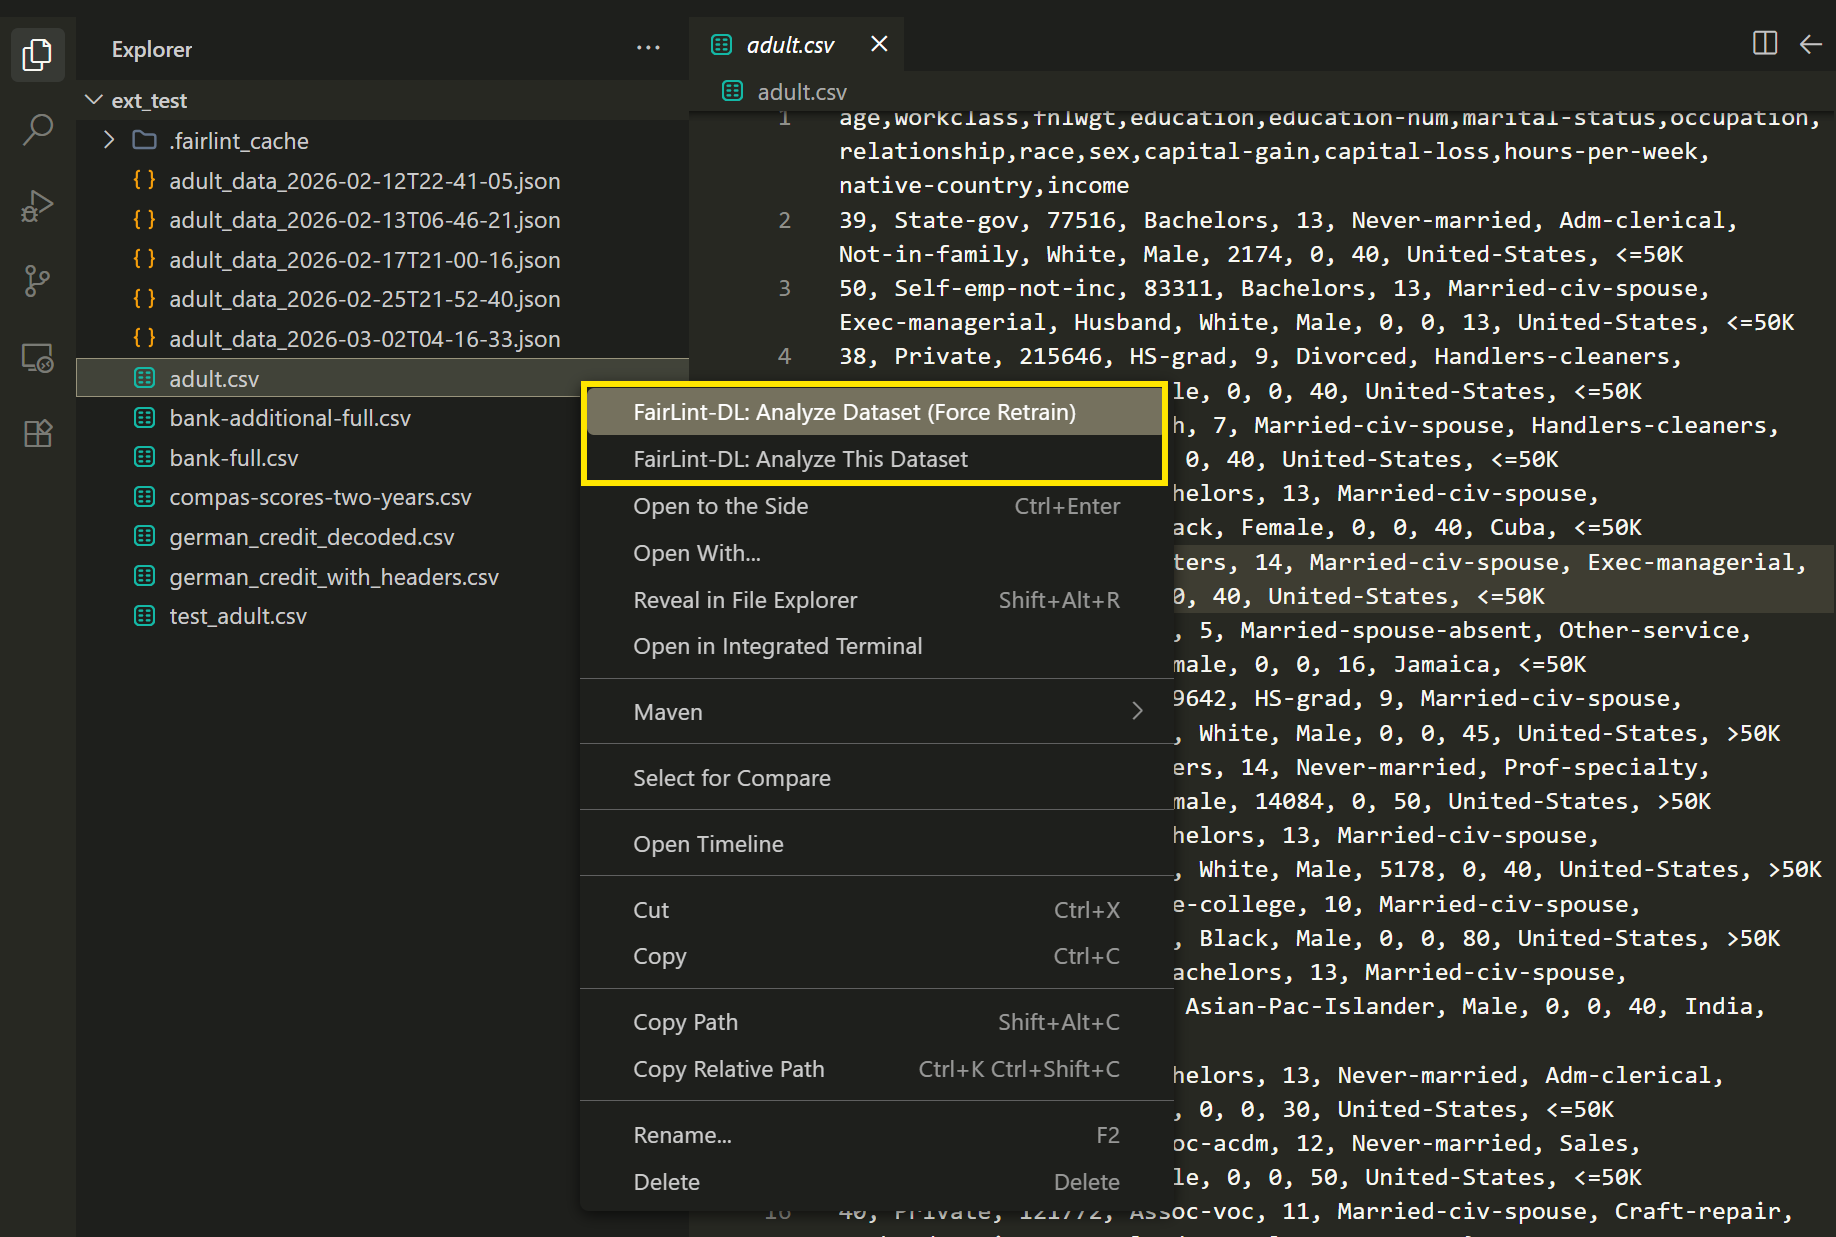
\includegraphics[width=0.95\textwidth]{images/context-menu-vscode.png}
    \caption{FairLint-DL context menu integration in VS Code.}
    \label{fig:vscode_menu}
\end{figure}

\chapter{Experimental Evaluation}
\label{ch:evaluation}

\section{Dataset: Adult Census Income}

The Adult Census Income dataset~\cite{adultdataset} (also known as the ``Census Income'' dataset) contains 32,561 records extracted from the 1994 U.S.\ Census Bureau database. The prediction task is binary classification: whether an individual's annual income exceeds \$50,000. The dataset contains 14 features and exhibits significant class imbalance, with 17,303 instances (53.2\%) in the low-income class and 5,489 instances (16.9\%) in the high-income class.

Four protected attributes were selected for analysis: \textbf{age} (71 unique values), \textbf{race} (5 unique values), \textbf{sex} (2 unique values), and \textbf{native-country} (42 unique values).

\begin{table}[H]
\centering
\caption{Dataset split and model configuration.}
\label{tab:dataset}
\begin{tabular}{@{}lr@{}}
\toprule
\textbf{Parameter} & \textbf{Value} \\
\midrule
Total instances & 32,561 \\
Training set & 22,792 (70\%) \\
Validation set & 3,256 (10\%) \\
Test set & 6,513 (20\%) \\
Number of features & 14 \\
Hidden layers & $\langle 64, 32, 16, 8, 4 \rangle$ \\
Output neurons & 2 (binary) \\
Total parameters & 3,998 \\
Epochs trained & 30 \\
\bottomrule
\end{tabular}
\end{table}

\section{Model Training Results}

The proxy model achieved 85.34\% test accuracy, with final training loss of 0.356 and validation loss of 0.324. The gap where test accuracy exceeds training accuracy (85.34\% vs.\ 83.32\%) is attributable to early stopping restoring the best validation-loss model state, combined with Dropout being disabled during evaluation.

\begin{figure}[H]
    \centering
    \fbox{\parbox{0.85\textwidth}{\centering\vspace{0.5cm}
    \textbf{[INSERT FIGURE: Training History Plot]}\\[0.3cm]
    \textit{Plot showing training loss/accuracy and validation loss/accuracy over 30 epochs, demonstrating convergence and the early stopping behavior.}
    \vspace{0.5cm}}}
    \caption{Training and validation curves over 30 epochs.}
    \label{fig:training}
\end{figure}

\section{QID Analysis Results}

Analysis of 500 randomly sampled test instances reveals pervasive individual discrimination:

\begin{table}[H]
\centering
\caption{QID analysis results on the Adult Census dataset.}
\label{tab:qid}
\begin{tabular}{@{}lr@{}}
\toprule
\textbf{Metric} & \textbf{Value} \\
\midrule
Instances analyzed & 500 \\
Mean QID (Shannon entropy) & 0.640 bits \\
Max QID & 1.000 bits \\
Standard deviation QID & 0.311 bits \\
Mean min-entropy QID & 0.214 bits \\
Mean disparate impact ratio & 0.581 \\
Discriminatory instances (QID $> 0.1$) & 479 (95.8\%) \\
Instances violating 80\% rule & 349 (69.8\%) \\
\bottomrule
\end{tabular}
\end{table}

A mean QID of 0.640 bits out of a theoretical maximum of 1.0 bit for binary classification indicates that protected attributes carry substantial influence over predictions. The near-universal discrimination rate of 95.8\% demonstrates that the model changes its prediction for nearly every individual when protected attributes are altered. The mean disparate impact ratio of 0.581 falls well below the 0.8 legal threshold.

\begin{figure}[H]
    \centering
    \fbox{\parbox{0.85\textwidth}{\centering\vspace{0.5cm}
    \textbf{[INSERT FIGURE: QID Distribution Histogram]}\\[0.3cm]
    \textit{Histogram showing the distribution of QID values across 500 analyzed instances, with the 0.1-bit threshold line and the concentration of values near the maximum.}
    \vspace{0.5cm}}}
    \caption{Distribution of QID values across 500 analyzed instances.}
    \label{fig:qid_dist}
\end{figure}

\section{Group Fairness Results}

Table~\ref{tab:group_fairness} presents the group fairness metrics across all four protected attributes.

\begin{table}[H]
\centering
\caption{Group fairness metrics by protected attribute.}
\label{tab:group_fairness}
\small
\begin{tabular}{@{}l c c c c c@{}}
\toprule
\textbf{Attribute} & \textbf{DP Diff} & \textbf{DP Ratio} & \textbf{TPR Diff} & \textbf{FPR Diff} & \textbf{EO Max} \\
\midrule
Sex & 0.162 & 0.298 & 0.088 & 0.065 & 0.088 \\
Age & 0.181 & 0.344 & 0.097 & 0.078 & 0.097 \\
Race & 0.083 & 0.564 & 0.086 & 0.025 & 0.086 \\
Native-country & 0.042 & 0.769 & 0.021 & 0.012 & 0.021 \\
\bottomrule
\end{tabular}
\end{table}

The \textbf{sex} attribute exhibits the most severe bias: a demographic parity ratio of 0.298 (far below the 0.8 threshold) indicates that Group~A (female, $n=2{,}158$) receives positive predictions at only 6.9\% compared to 23.1\% for Group~B (male, $n=4{,}355$). The \textbf{age} attribute shows similarly concerning disparities with a DP ratio of 0.344. The \textbf{race} attribute has moderate bias (DP ratio 0.564), while \textbf{native-country} shows the least disparity (DP ratio 0.769, approaching fairness).

\begin{figure}[H]
    \centering
    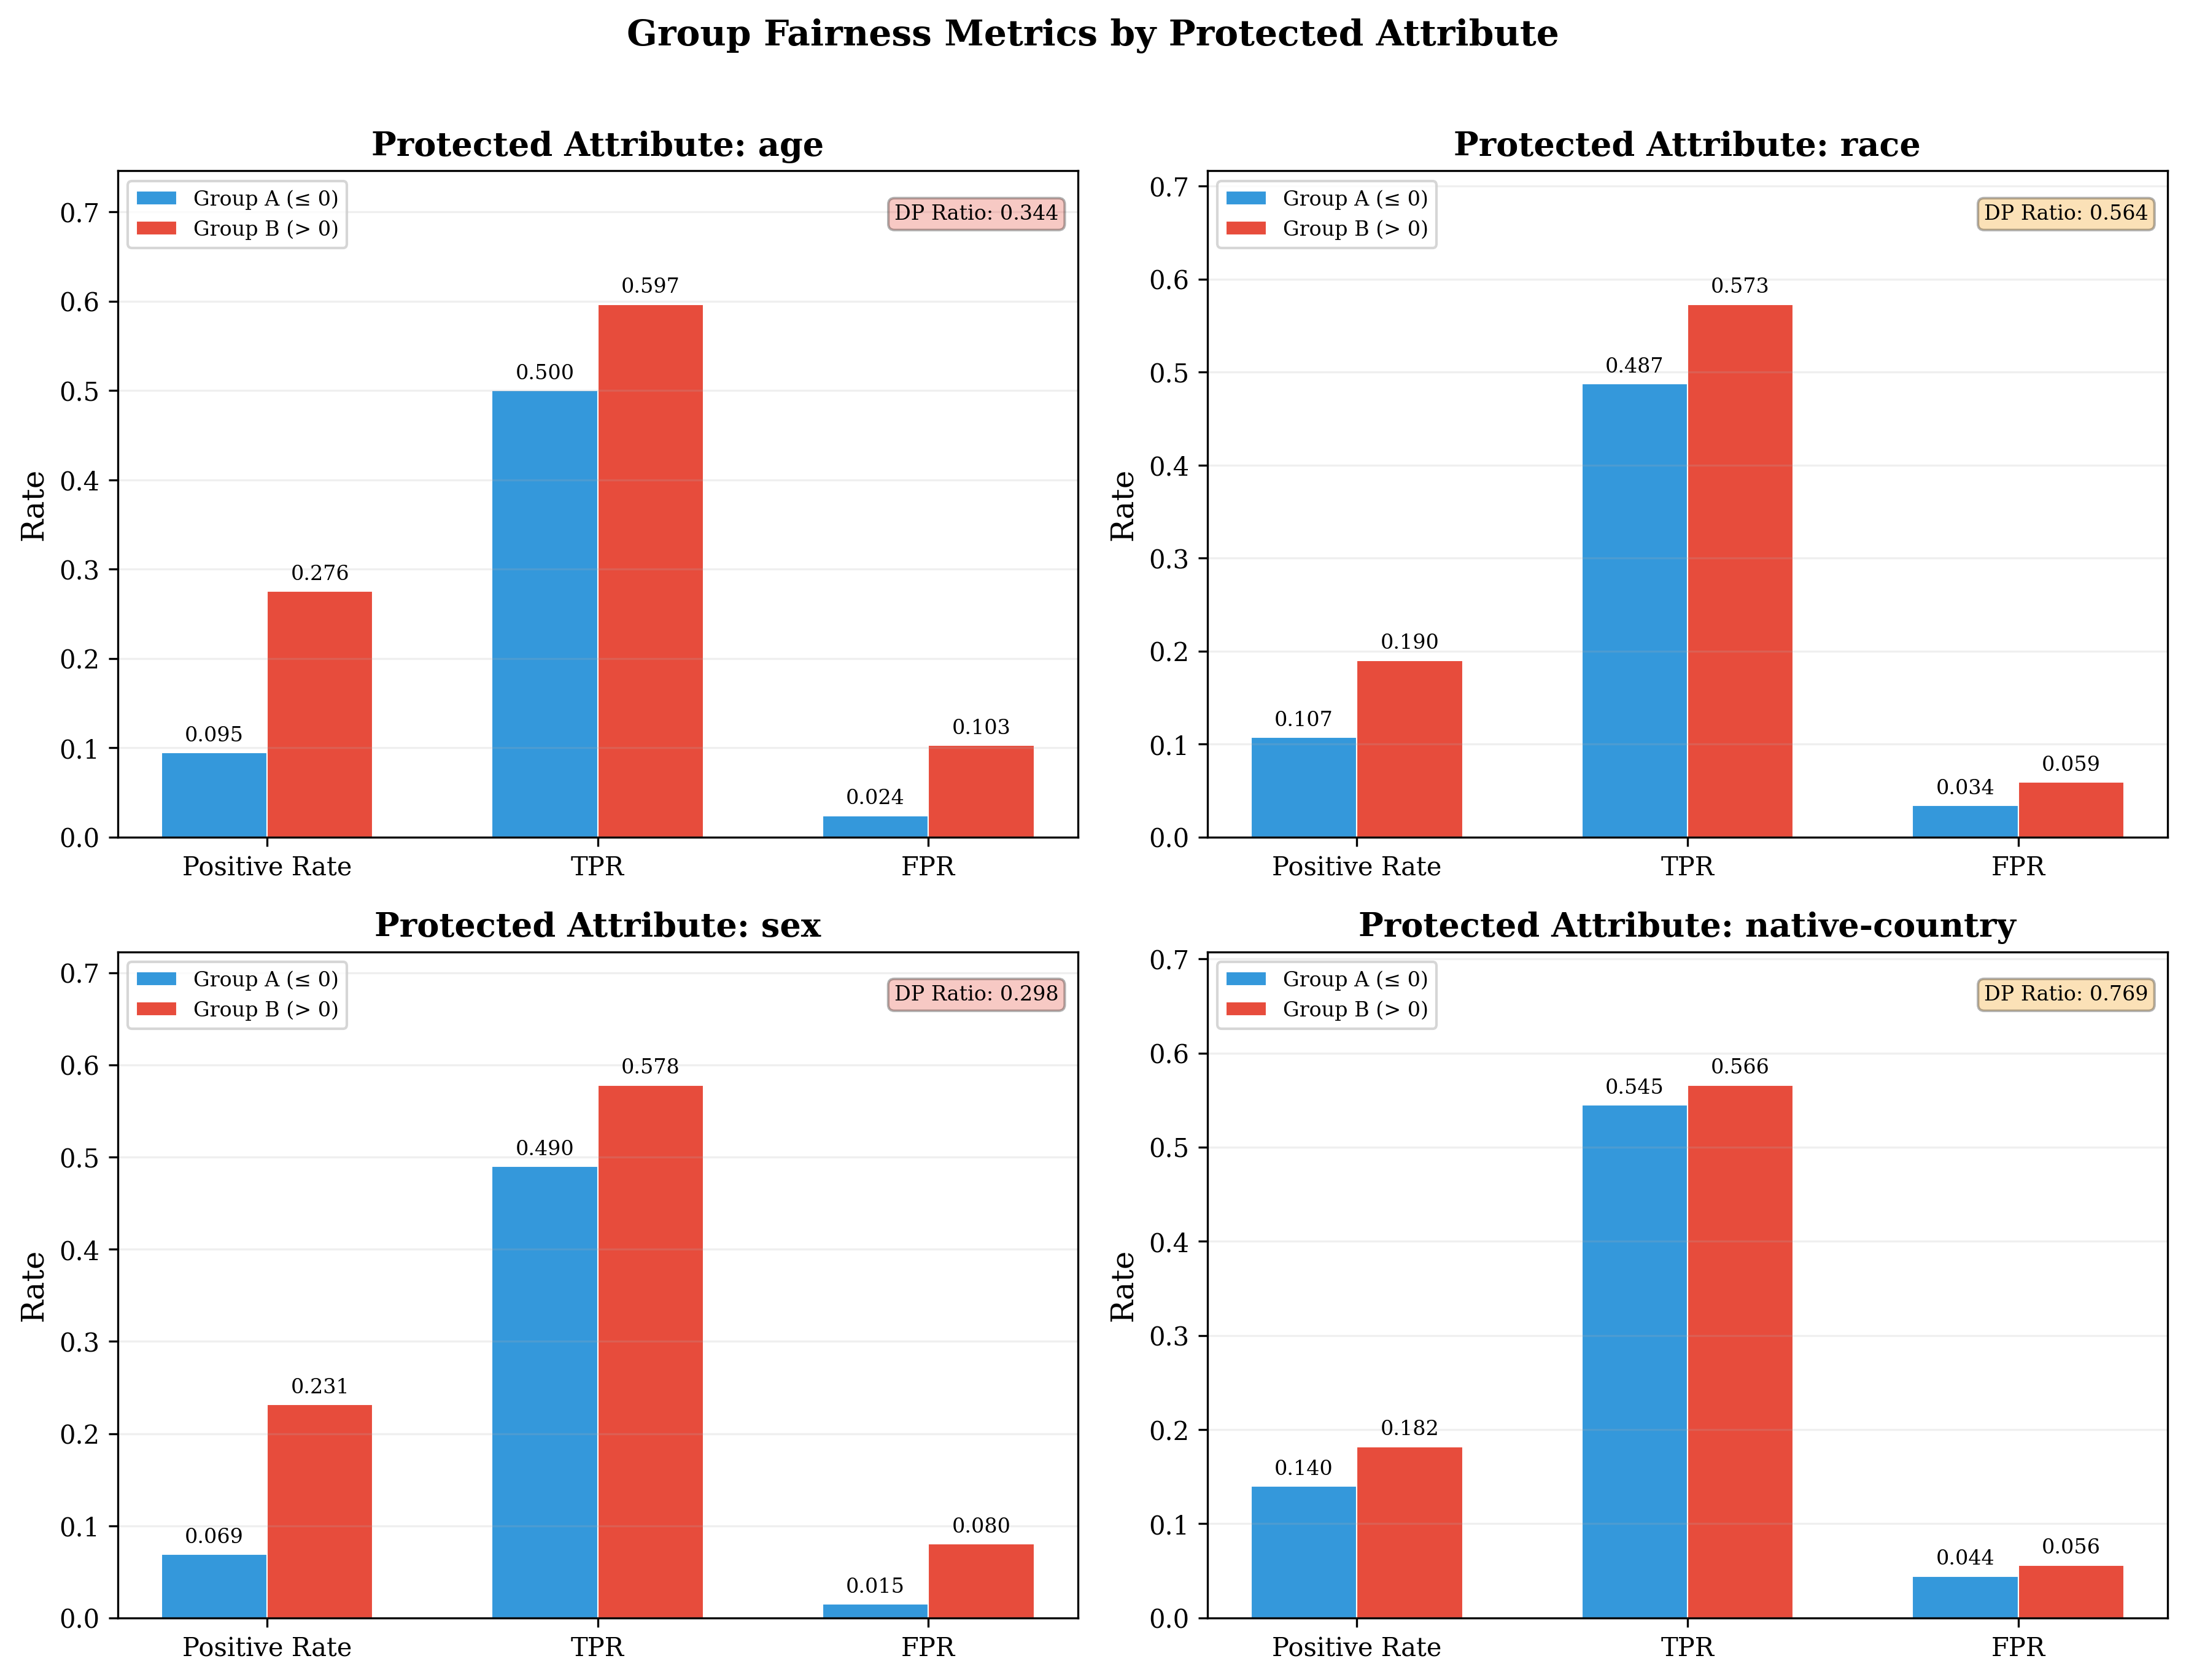
\includegraphics[width=0.95\textwidth]{images/group-fairness.png}
    \caption{Group fairness metric comparisons across protected attributes.}
    \label{fig:group_fairness}
\end{figure}

\section{Discriminatory Instance Search Results}

The gradient-guided search discovered 30 discriminatory instances. The best QID found during global search was 0.011 bits, which appears low compared to the mean QID of 0.640 bits because the search explores synthetic input regions rather than natural data instances---the search finds the input configuration where the model's counterfactual predictions are most extreme.

\section{Causal Debugging Results}

\subsection{Layer Sensitivity Analysis}

Table~\ref{tab:layer_sensitivity} presents the layer-by-layer sensitivity scores.

\begin{table}[H]
\centering
\caption{Layer sensitivity analysis results.}
\label{tab:layer_sensitivity}
\begin{tabular}{@{}lccc@{}}
\toprule
\textbf{Layer} & \textbf{Neurons} & \textbf{Sensitivity} & \textbf{Relative} \\
\midrule
Layer 1 & 64 & 1.443 & 74.7\% \\
\textbf{Layer 2} & \textbf{32} & \textbf{1.933} & \textbf{100.0\%} \\
Layer 3 & 16 & 0.769 & 39.8\% \\
Layer 4 & 8 & 0.191 & 9.9\% \\
Layer 5 & 4 & 0.188 & 9.7\% \\
Layer 6 (Output) & 2 & 0.124 & 6.4\% \\
\bottomrule
\end{tabular}
\end{table}

\textbf{Layer 2} (32 neurons) is identified as the most bias-sensitive layer with a sensitivity score of 1.933, indicating that this layer amplifies protected attribute information most strongly. Bias concentrated in early-to-middle layers suggests the network encodes protected information during initial feature transformation before it propagates through deeper layers. This finding is consistent with the causal debugging results reported by DICE~\cite{dice} on the same Adult Census dataset, which similarly identified the second layer as the most bias-sensitive.

\begin{figure}[H]
    \centering
    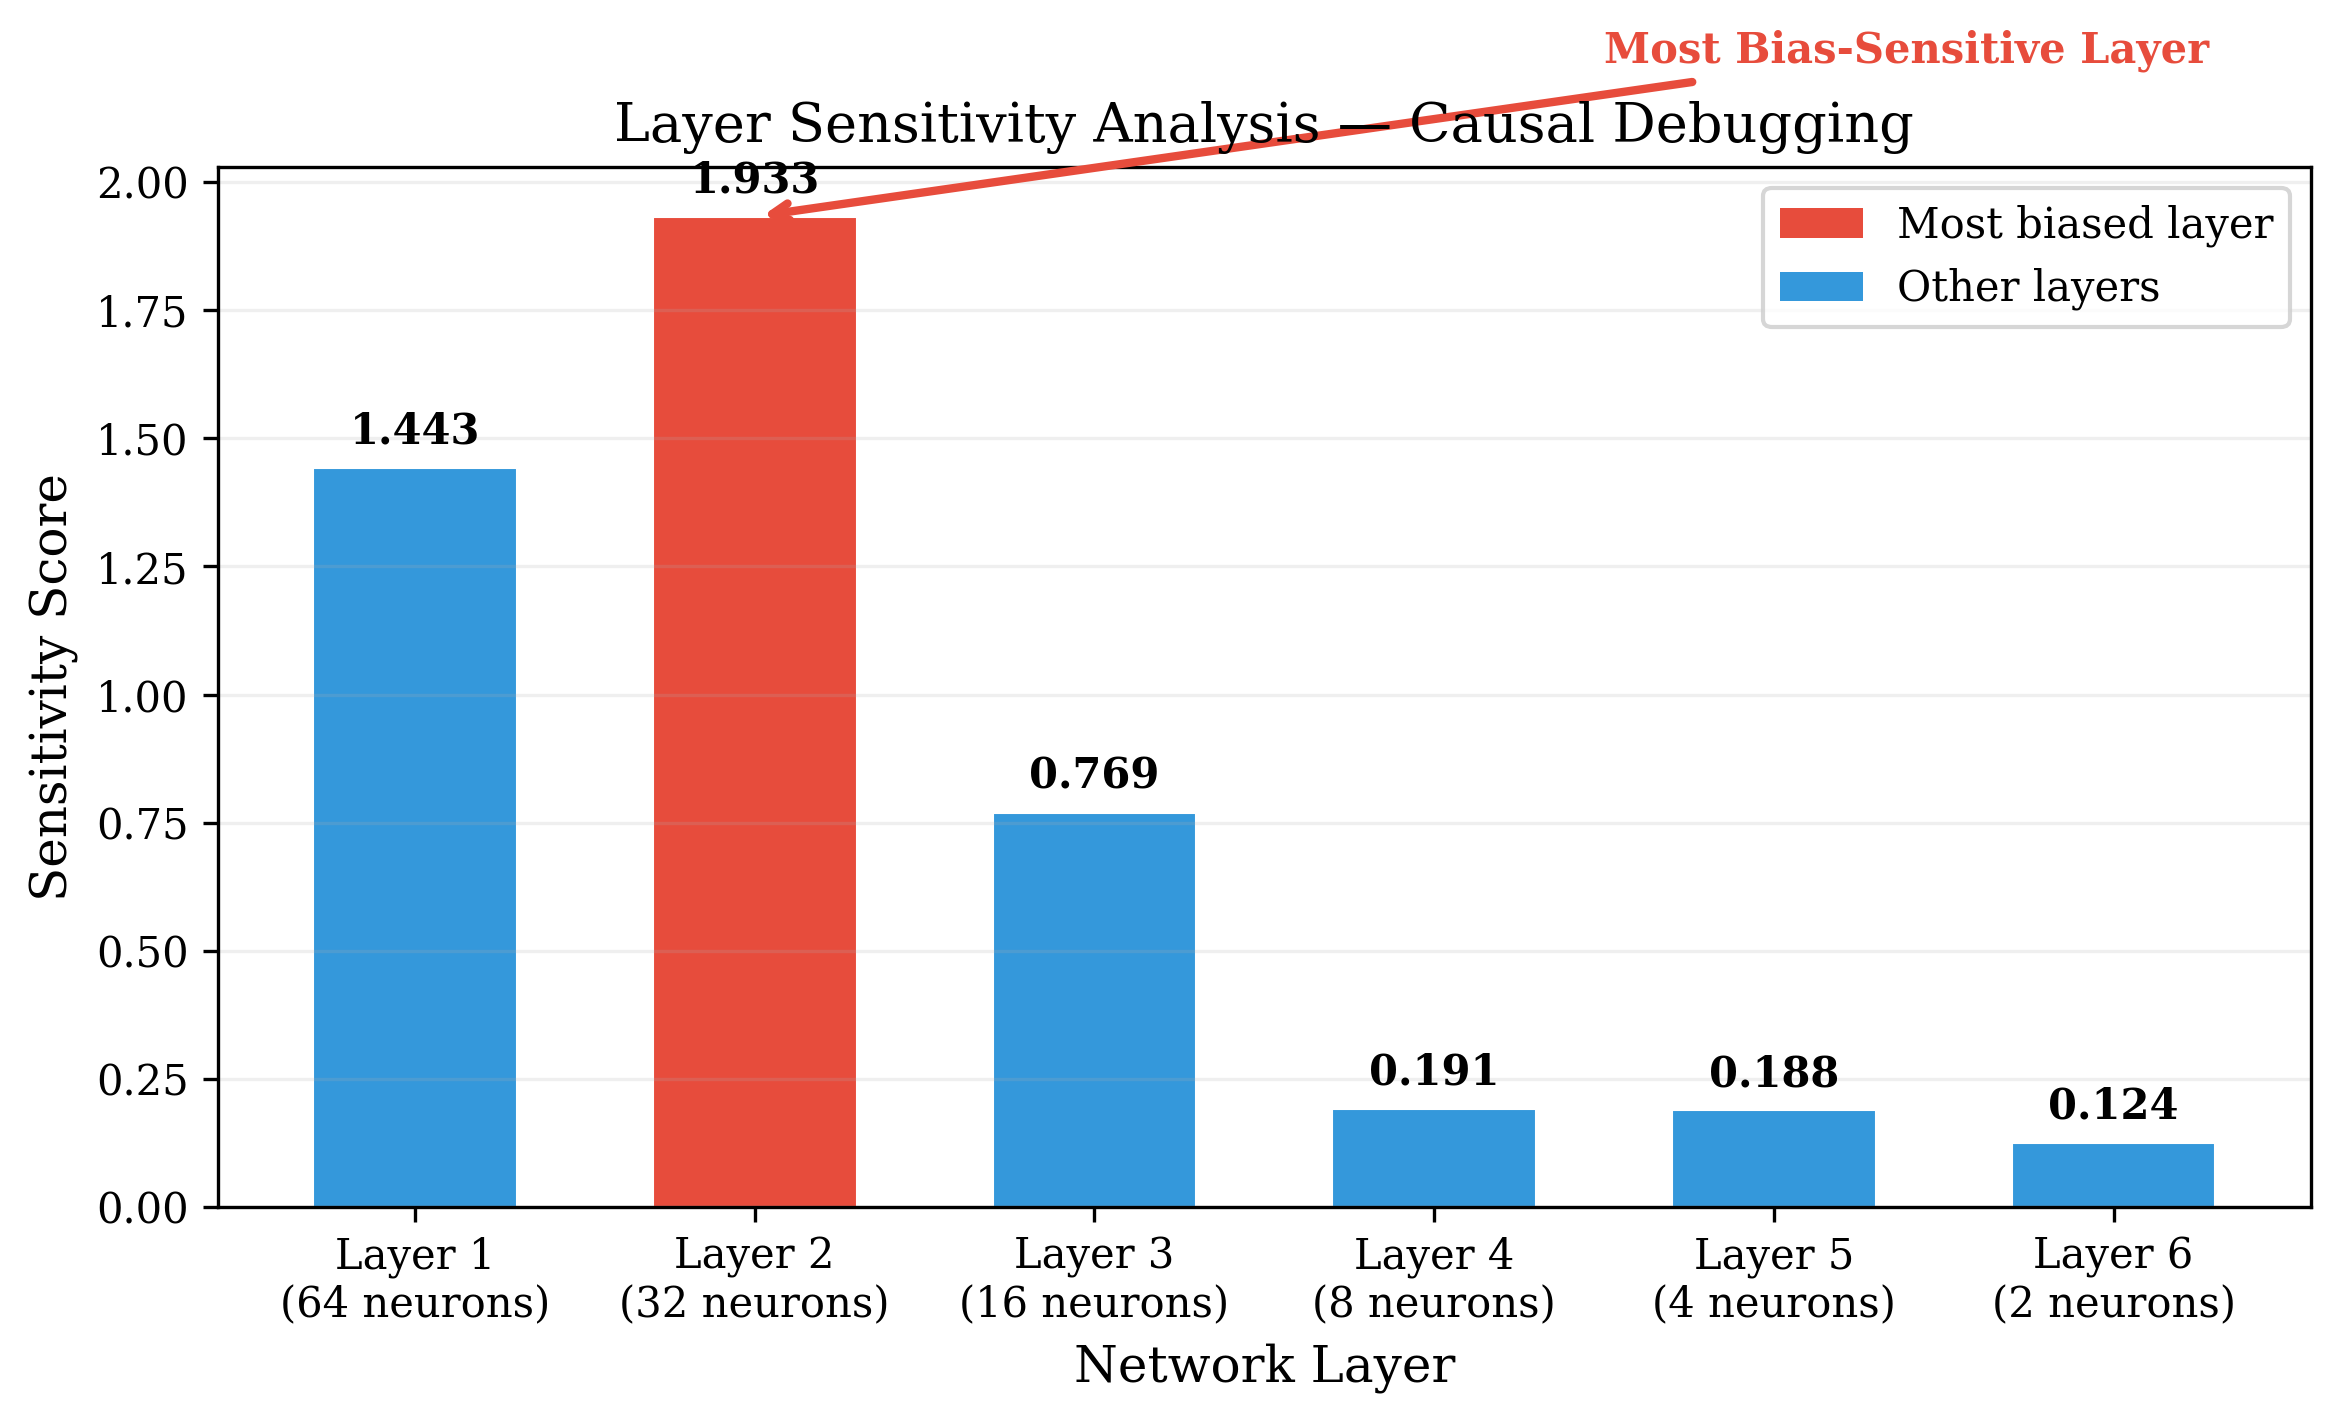
\includegraphics[width=0.95\textwidth]{images/layer-sensitivity.png}
    \caption{Layer sensitivity analysis identifying Layer 2 as the bias-critical layer.}
    \label{fig:layer_sensitivity}
\end{figure}

\subsection{Neuron-Level Analysis}

Within Layer~2, the top 5 biased neurons are:

\begin{table}[H]
\centering
\caption{Top 5 biased neurons in Layer 2.}
\label{tab:neurons}
\begin{tabular}{@{}lcc@{}}
\toprule
\textbf{Neuron} & \textbf{Impact Score} & \textbf{Relative} \\
\midrule
Neuron 30 & 1.362 & 100.0\% \\
Neuron 17 & 1.270 & 93.3\% \\
Neuron 8 & 1.220 & 89.6\% \\
Neuron 29 & 1.055 & 77.5\% \\
Neuron 23 & 0.985 & 72.3\% \\
\bottomrule
\end{tabular}
\end{table}

Neurons 30 and 17 have disproportionately high impact scores, suggesting they have specialized in encoding protected attribute information. In a fairness remediation workflow, these neurons would be primary candidates for neuron-level dropout interventions as proposed by NeuFair~\cite{neufair}.

\begin{figure}[H]
    \centering
    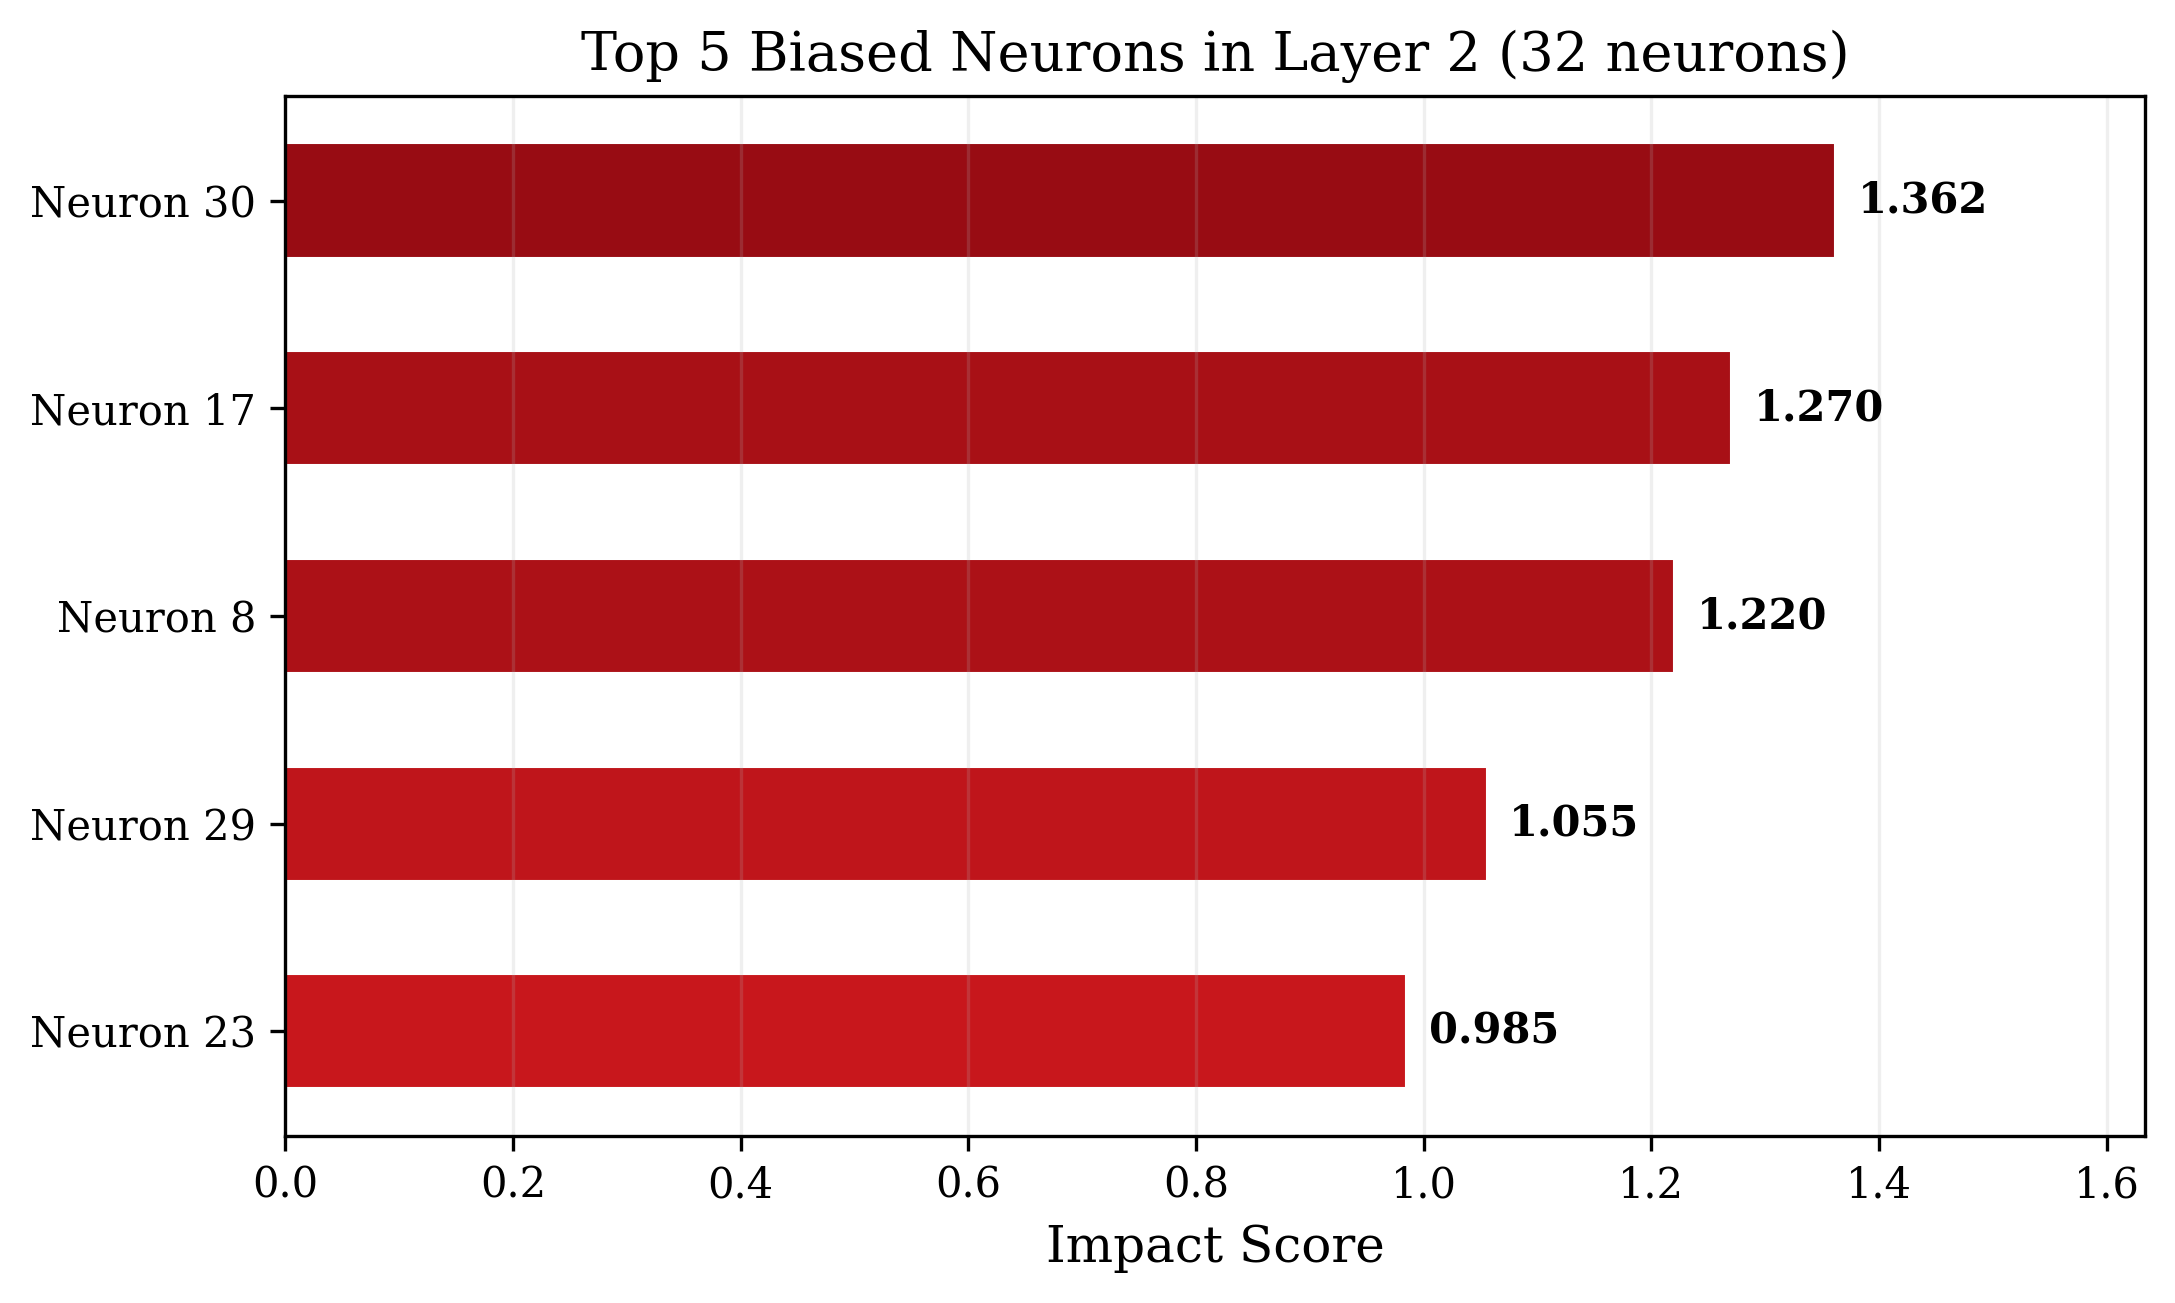
\includegraphics[width=0.95\textwidth]{images/neuron-impact.png}
    \caption{Neuron-level impact scores within Layer 2.}
    \label{fig:neuron_impact}
\end{figure}

\section{Explainability Results}

\subsection{SHAP Global Feature Importance}

Table~\ref{tab:shap} presents the SHAP global feature importance values computed on the log-odds output space.

\begin{table}[H]
\centering
\caption{SHAP global feature importance (log-odds space).}
\label{tab:shap}
\begin{tabular}{@{}clc@{}}
\toprule
\textbf{Rank} & \textbf{Feature} & \textbf{Importance} \\
\midrule
1 & education-num & 0.891 \\
2 & age$^\dagger$ & 0.690 \\
3 & marital-status & 0.688 \\
4 & hours-per-week & 0.541 \\
5 & capital-gain & 0.326 \\
6 & capital-loss & 0.233 \\
7 & relationship & 0.251 \\
8 & sex$^\dagger$ & 0.176 \\
9 & occupation & 0.115 \\
10 & education & 0.108 \\
\bottomrule
\multicolumn{3}{@{}l}{\footnotesize $^\dagger$ Protected attribute.}
\end{tabular}
\end{table}

Notably, \textbf{age} (a protected attribute) ranks \#2 in global importance, confirming that the model heavily relies on age information for predictions. \textbf{Sex} ranks \#8, indicating moderate but measurable influence. \textbf{Race} (importance: 0.010) and \textbf{native-country} (importance: 0.000) show minimal direct SHAP influence, though this does not preclude indirect influence through correlated proxy features.

\subsection{LIME Aggregated Feature Importance}

\begin{table}[H]
\centering
\caption{LIME aggregated feature importance (top 5).}
\label{tab:lime}
\begin{tabular}{@{}clc@{}}
\toprule
\textbf{Rank} & \textbf{Feature} & \textbf{Importance} \\
\midrule
1 & capital-gain & 0.246 \\
2 & education-num & 0.232 \\
3 & marital-status & 0.159 \\
4 & capital-loss & 0.156 \\
5 & hours-per-week & 0.128 \\
\bottomrule
\end{tabular}
\end{table}

Both SHAP and LIME agree that \textbf{education-num} is among the most important features, and both identify \textbf{age} as a significant protected attribute with measurable influence. This cross-method agreement provides high confidence in the feature attribution findings.

\begin{figure}[H]
    \centering
    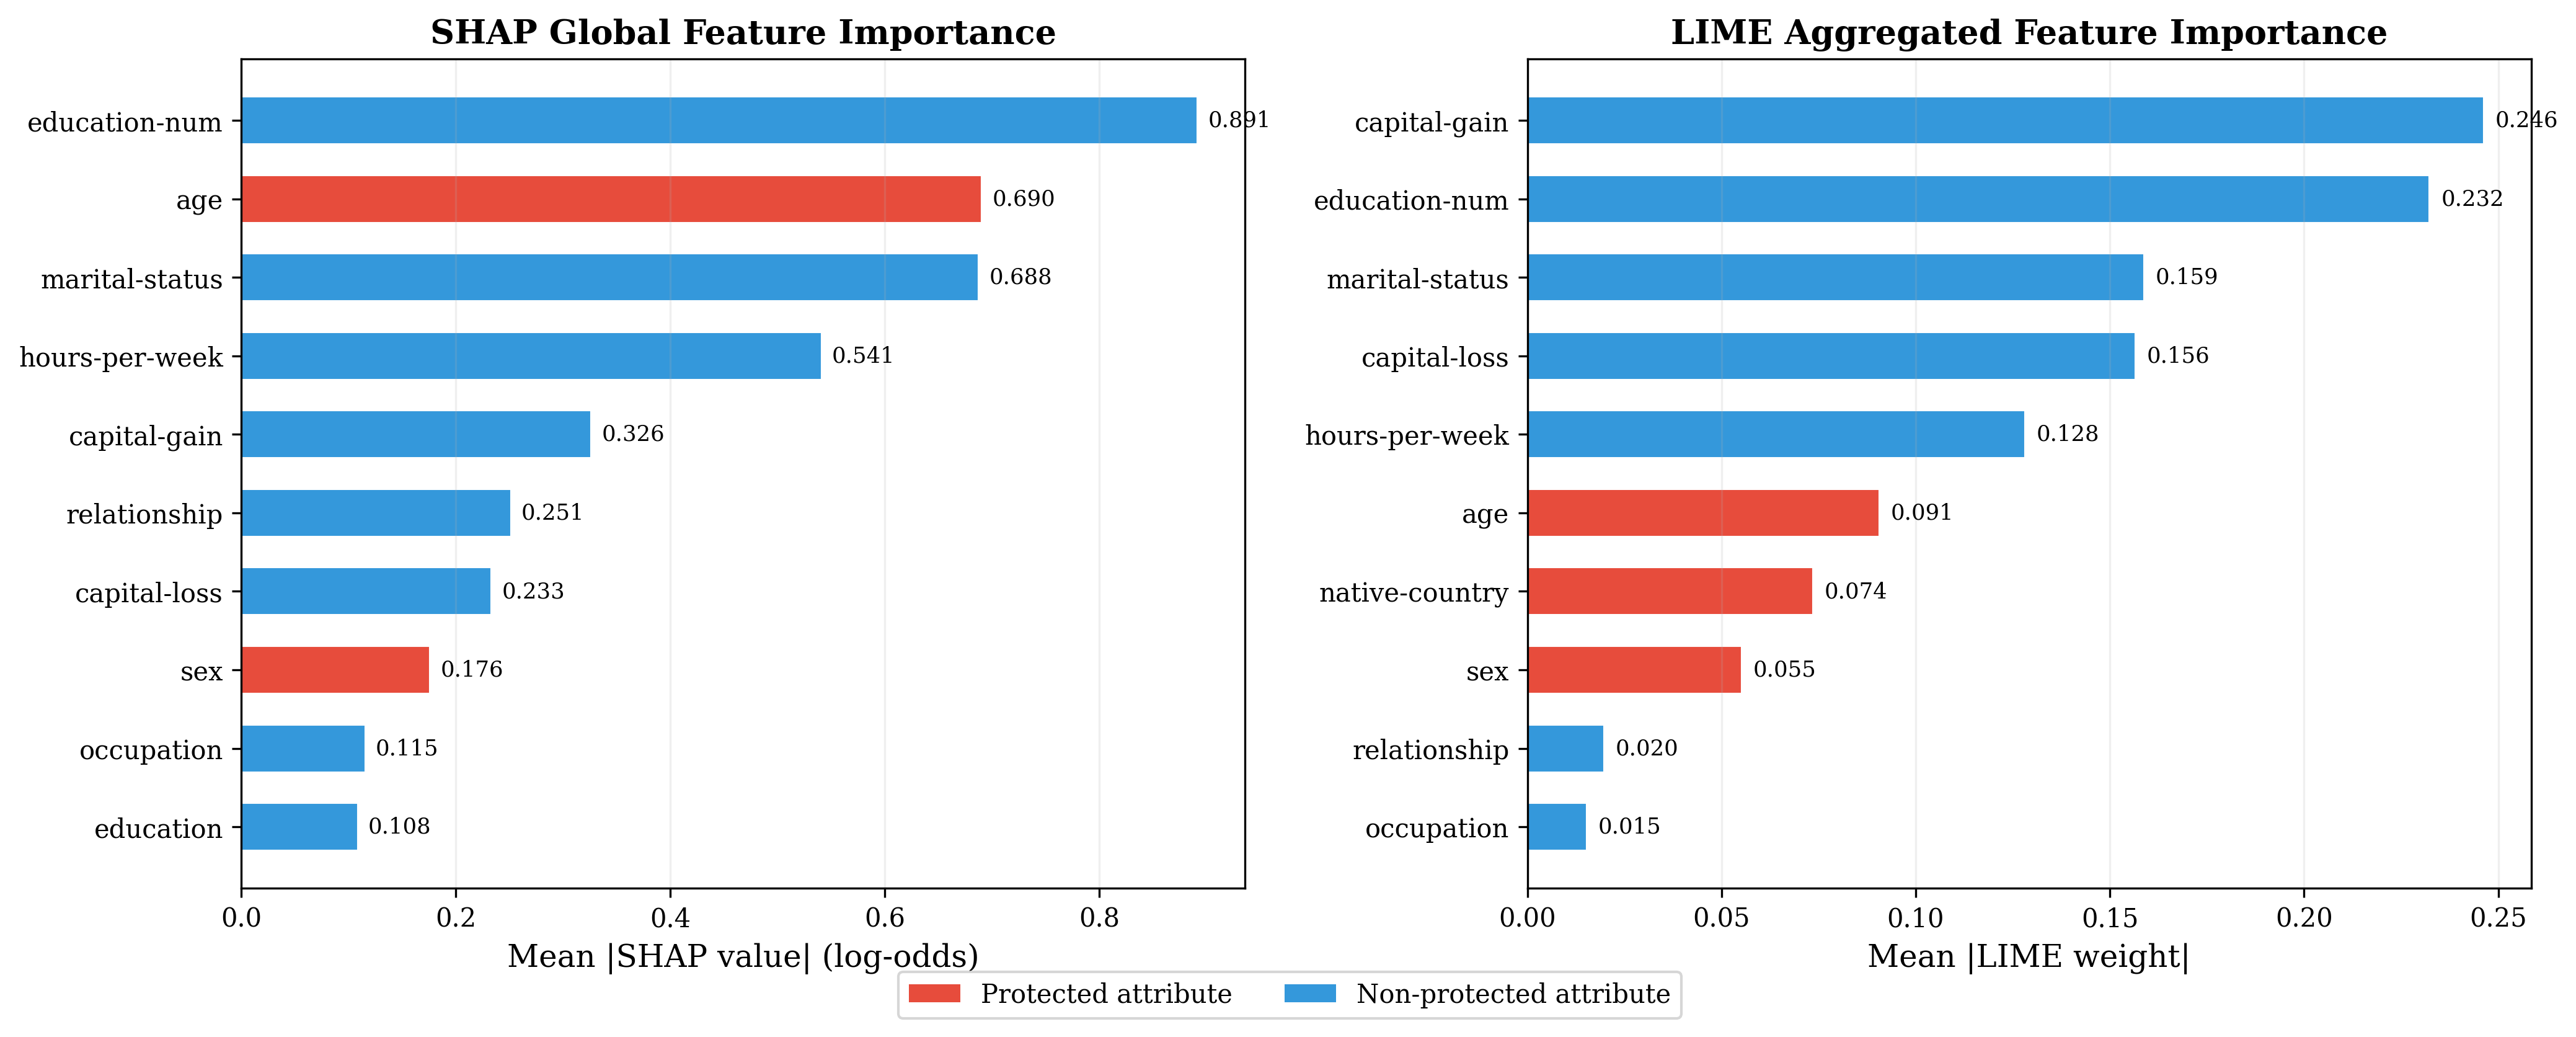
\includegraphics[width=0.95\textwidth]{images/shap-lime.png}
    \caption{SHAP and LIME feature importance comparison.}
    \label{fig:explainability}
\end{figure}

\section{Composite Fairness Score}

Applying the scoring formula from Equation~\ref{eq:score}:

\begin{table}[H]
\centering
\caption{Composite fairness score breakdown.}
\label{tab:score}
\begin{tabular}{@{}lrrr@{}}
\toprule
\textbf{Component} & \textbf{Value} & \textbf{Calculation} & \textbf{Penalty} \\
\midrule
Mean QID & 0.640 bits & $0.640 \times 15 = 9.60$ & $-10$ \\
\% Discriminatory & 95.8\% & $95.8 \times 0.3 = 28.74$ & $-29$ \\
Disparate Impact & 0.581 & $(0.8 - 0.581) \times 50 = 10.95$ & $-11$ \\
Max QID & 1.000 bits & $1.0 \times 5 = 5.0$ & $-5$ \\
Group Fairness & averaged & $(\bar{\text{DP}} + \bar{\text{EO}}) \times 25$ & $\sim$$-5$ \\
\midrule
\textbf{Total Score} & & $100 - 10 - 29 - 11 - 5 - 5$ & $\approx \mathbf{41}$ \\
\bottomrule
\end{tabular}
\end{table}

The final score of approximately \textbf{41 out of 100} is rated \textbf{``Concerning''} (red), indicating significant bias that would require substantial remediation before deployment.

\begin{figure}[H]
    \centering
    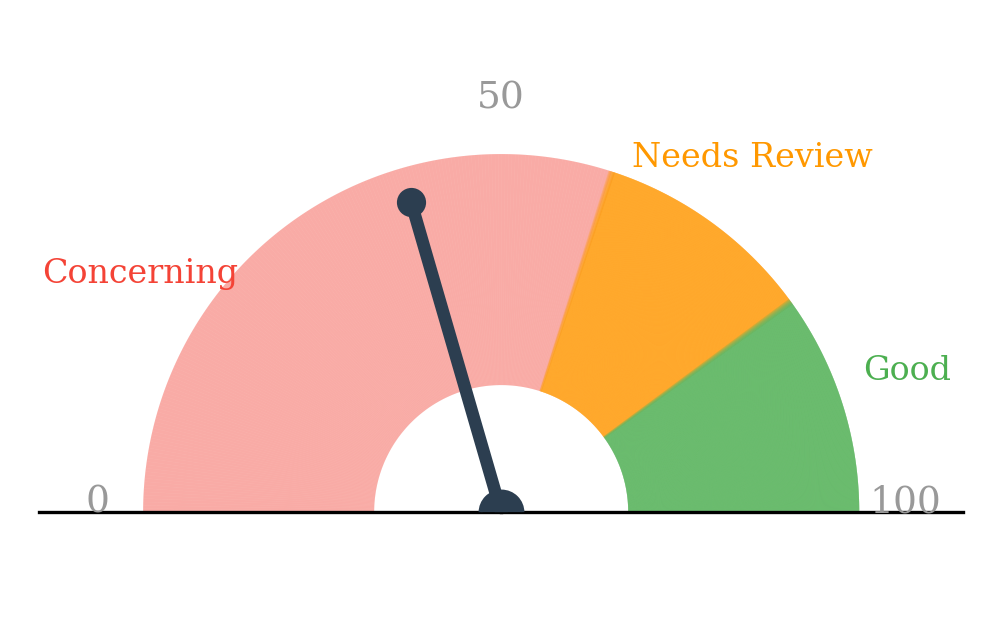
\includegraphics[width=0.95\textwidth]{images/fairness-gauge.png}
    \caption{Composite fairness score gauge for the Adult Census dataset.}
    \label{fig:gauge}
\end{figure}

\section{Performance Timing}

\begin{table}[H]
\centering
\caption{Analysis pipeline timing (cached model).}
\label{tab:timing}
\begin{tabular}{@{}lr@{}}
\toprule
\textbf{Step} & \textbf{Duration (s)} \\
\midrule
Model Training (cached) & 1 \\
Activations & 1 \\
QID Analysis + Group Fairness & 1 \\
Discriminatory Instance Search & 2 \\
Causal Debugging & $<$1 \\
SHAP + LIME Explanations & 7 \\
\midrule
\textbf{Total} & \textbf{12} \\
\bottomrule
\end{tabular}
\end{table}

With model caching, the full analysis completes in approximately 12 seconds, demonstrating the feasibility of integrating comprehensive fairness analysis into the developer workflow. First-run training adds approximately 77 seconds for the Adult Census dataset.

\chapter{Discussion}
\label{ch:discussion}

\section{Interpretation of Results}

The Adult Census dataset exhibits significant and pervasive fairness concerns when analyzed through FairLint-DL's deep neural network proxy model. Five key findings emerge:

\textbf{(1) Pervasive individual discrimination:} 95.8\% of analyzed instances show QID above the 0.1-bit threshold, meaning the model changes its prediction for nearly every individual when protected attributes are altered. This is not an isolated phenomenon affecting edge cases but a systemic property of the learned decision boundary.

\textbf{(2) High average bias:} A mean QID of 0.640 bits (out of a maximum of 1.0 for binary classification) indicates that protected attributes carry substantial influence over predictions---more than half the theoretical maximum information leakage.

\textbf{(3) Legal threshold violations:} 69.8\% of instances violate the four-fifths rule (disparate impact $< 0.8$), suggesting the model would likely fail legal scrutiny for disparate impact under U.S.\ civil rights law.

\textbf{(4) Group-level disparities:} Sex and age exhibit the most severe group-level bias. The demographic parity ratio of 0.298 for sex means females receive favorable predictions at less than one-third the rate of males. This reflects well-documented historical income disparities embedded in the training data.

\textbf{(5) Bias localization:} Causal debugging identifies Layer~2 as the bias-critical layer, with specific neurons (30 and 17) encoding protected information. This localization enables targeted remediation strategies such as selective neuron dropout~\cite{neufair} or regularization, rather than wholesale model retraining.

\section{Cross-Method Validation}

The agreement between SHAP and LIME on the importance of education-num and age provides robust evidence for these findings. Interestingly, while race shows minimal direct SHAP importance (0.010), the QID analysis reveals significant discrimination across racial groups (DP ratio: 0.564). This discrepancy suggests that race influences predictions indirectly through correlated proxy features---a form of proxy discrimination that is particularly insidious because it may not be detected by single-method analysis.

\section{Sources of Bias}

The bias detected in the Adult Census dataset stems from multiple sources along the data lifecycle~\cite{barocas-hardt-narayanan}:

\textbf{Pre-data bias:} Historical income inequality between demographic groups (historical bias, structural inequality) is directly encoded in the training labels.

\textbf{Data processing bias:} Proxy variables such as occupation, relationship status, and hours-per-week are strongly correlated with protected attributes, creating indirect pathways for discrimination (proxy discrimination, Simpson's paradox).

\textbf{Model bias:} The DNN's optimization objective (cross-entropy loss) maximizes overall accuracy without fairness constraints, leading to disparate performance across demographic subgroups (evaluation bias, objective function bias).

\section{Limitations}

\textbf{Proxy model limitation:} FairLint-DL trains its own DNN proxy model rather than analyzing an externally provided model. The bias detected reflects the proxy model's behavior, which may differ from a production model trained with different architectures or fairness constraints.

\textbf{Group definition:} Using standardized values ($\leq 0$ vs.\ $> 0$) for group splitting is appropriate for binary attributes (sex) but may not capture meaningful group boundaries for continuous attributes (age) or multi-class attributes (race with 5 categories).

\textbf{Single-dataset evaluation:} This report evaluates FairLint-DL on a single benchmark dataset. While the Adult Census dataset is widely used in fairness research, evaluation on additional datasets (COMPAS, German Credit, Bank Marketing) would strengthen the generalizability claims.

\textbf{Scalability:} SHAP's KernelExplainer has quadratic complexity in the number of features, making it the computational bottleneck (7 seconds of the 12-second total). For datasets with many features, this may require sampling-based approximations.


\chapter{Conclusion and Future Work}
\label{ch:conclusion}

\section{Conclusion}

This report presented FairLint-DL, a VS Code extension for deep learning-based fairness debugging of machine learning datasets. By implementing the shift-left fairness testing paradigm, FairLint-DL enables practitioners to detect, quantify, localize, and explain bias directly within their development environment---before committing to production model architectures.

The system integrates information-theoretic QID metrics, gradient-guided discriminatory instance search, causal debugging with layer and neuron localization, group fairness metrics (Demographic Parity, Equalized Odds, Equal Opportunity), and dual SHAP/LIME explainability into a cohesive six-step analysis pipeline~\cite{dice, neufair}. Evaluation on the Adult Census Income dataset demonstrates both the severity of bias in commonly used benchmark data and the effectiveness of FairLint-DL's multi-faceted analysis approach.

The composite fairness score of approximately 41/100 for the Adult Census dataset, combined with the identification of Layer~2 Neurons~30 and~17 as primary bias drivers and the cross-validated SHAP/LIME feature attributions, provides practitioners with actionable intelligence for fairness remediation. The 12-second analysis time (with cached models) makes iterative fairness assessment practical within the development workflow.

\section{Future Work}

Several directions for future research and development emerge from this work:

\textbf{Model retraining with fairness constraints:} Integrating in-processing fairness interventions such as adversarial debiasing, fairness-constrained optimization~\cite{agarwal2018}, or the NeuFair dropout strategy~\cite{neufair} directly into the extension, enabling a closed-loop ``detect--fix--verify'' workflow.

\textbf{Neuron-level interventions:} Implementing selective neuron pruning or activation clamping for the identified bias-critical neurons, guided by the causal debugging results, with real-time fairness score updates.

\textbf{Multi-dataset validation:} Extending evaluation to COMPAS (criminal justice), German Credit (lending), Bank Marketing (financial services), and MEPS (healthcare) datasets to validate generalizability across domains.

\textbf{Intersectional fairness:} Analyzing bias across combinations of protected attributes (e.g., race $\times$ gender $\times$ age) to capture intersectional discrimination that single-attribute analysis may miss~\cite{barocas-hardt-narayanan}.

\textbf{Real-time monitoring:} Extending FairLint-DL for continuous fairness monitoring during model development, with automated alerts when fairness metrics degrade below configurable thresholds.

\textbf{Alternative model architectures:} Supporting external model analysis (not just proxy models) and extending to non-tabular data domains including NLP (LLM bias) and computer vision (representation bias).


% appendices
\appendices
\appendix\chapter{}\label{app:dashboard}
\appendixtitle{Full Results Dashboard}

\begin{figure}[H]
    \centering
    \fbox{\parbox{0.85\textwidth}{\centering\vspace{0.8cm}
    \textbf{[INSERT FIGURE: Full Dashboard Screenshot --- Overview Section]}\\[0.3cm]
    \textit{Full-width screenshot of the FairLint-DL dashboard showing the pipeline overview, dataset summary, protected attributes, and fairness score gauge.}
    \vspace{0.7cm}}}
    \caption{FairLint-DL dashboard: Pipeline overview and fairness score.}
    \label{fig:dashboard_overview}
\end{figure}

\begin{figure}[H]
    \centering
    \fbox{\parbox{0.85\textwidth}{\centering\vspace{0.8cm}
    \textbf{[INSERT FIGURE: Full Dashboard Screenshot --- QID Section]}\\[0.3cm]
    \textit{Screenshot of the QID analysis section showing mean/max/std QID values, discrimination percentage, disparate impact ratio, and the QID distribution histogram.}
    \vspace{0.7cm}}}
    \caption{FairLint-DL dashboard: QID analysis section.}
    \label{fig:dashboard_qid}
\end{figure}

\begin{figure}[H]
    \centering
    \fbox{\parbox{0.85\textwidth}{\centering\vspace{0.8cm}
    \textbf{[INSERT FIGURE: Full Dashboard Screenshot --- Group Fairness Section]}\\[0.3cm]
    \textit{Screenshot showing the group fairness metrics with attribute selector, DP/EO/EOpp metric cards with Fair/Marginal/Unfair badges, and per-group comparison charts.}
    \vspace{0.7cm}}}
    \caption{FairLint-DL dashboard: Group fairness metrics section.}
    \label{fig:dashboard_group}
\end{figure}

\begin{figure}[H]
    \centering
    \fbox{\parbox{0.85\textwidth}{\centering\vspace{0.8cm}
    \textbf{[INSERT FIGURE: Full Dashboard Screenshot --- Causal Debugging Section]}\\[0.3cm]
    \textit{Screenshot showing the layer sensitivity bar chart, most biased layer identification, and neuron impact bar chart with interpretive text.}
    \vspace{0.7cm}}}
    \caption{FairLint-DL dashboard: Causal debugging section.}
    \label{fig:dashboard_causal}
\end{figure}

\begin{figure}[H]
    \centering
    \fbox{\parbox{0.85\textwidth}{\centering\vspace{0.8cm}
    \textbf{[INSERT FIGURE: Full Dashboard Screenshot --- SHAP/LIME Section]}\\[0.3cm]
    \textit{Screenshot showing the SHAP global importance bar chart, beeswarm plot, LIME aggregated importance, and the interactive LIME explorer with a per-instance explanation.}
    \vspace{0.7cm}}}
    \caption{FairLint-DL dashboard: SHAP and LIME explainability section.}
    \label{fig:dashboard_explain}
\end{figure}

\begin{figure}[H]
    \centering
    \fbox{\parbox{0.85\textwidth}{\centering\vspace{0.8cm}
    \textbf{[INSERT FIGURE: Internal Space Visualization]}\\[0.3cm]
    \textit{PCA scatter plots for each layer showing how the network separates data points, colored by protected attribute values. Observe the increasing separation in deeper layers.}
    \vspace{0.7cm}}}
    \caption{Internal space PCA visualization across network layers.}
    \label{fig:internal_space}
\end{figure}

\chapter{}\label{app:confusion}
\appendixtitle{Confusion Matrices}

\begin{table}[H]
\centering
\caption{Per-group confusion matrices for all protected attributes.}
\label{tab:confusion}
\small
\begin{tabular}{@{}ll rrrr rrrr@{}}
\toprule
& & \multicolumn{4}{c}{\textbf{Group A ($\leq 0$)}} & \multicolumn{4}{c}{\textbf{Group B ($> 0$)}} \\
\cmidrule(lr){3-6} \cmidrule(lr){7-10}
\textbf{Attribute} & \textbf{Size} & TP & FP & TN & FN & TP & FP & TN & FN \\
\midrule
Age & 3531/2982 & 262 & 73 & 2934 & 262 & 623 & 199 & 1739 & 421 \\
Race & 980/5533 & 77 & 28 & 794 & 81 & 808 & 244 & 3879 & 602 \\
Sex & 2158/4355 & 120 & 29 & 1884 & 125 & 765 & 243 & 2789 & 558 \\
Native-c. & 644/5869 & 67 & 23 & 498 & 56 & 818 & 249 & 4175 & 627 \\
\bottomrule
\end{tabular}
\end{table}


% references
\bibformb
\bibliography{src/bibphd.bib}

\makeatother
\end{document}
